\chapter{Research Outcomes}

\section{Overview}
This chapter presents a comprehensive analysis of RE-TabSyn's performance against baseline methods across six financial datasets. We examine statistical fidelity, machine learning utility, privacy preservation, and the critical capability of minority class control. All results are reported as mean $\pm$ standard deviation across three random seeds (42, 123, 456) to establish statistical significance. The evaluation uses the three-pillar framework (Fidelity, Utility, Privacy) described in Chapter 4.

\section{Statistical Similarity Analysis}
Statistical fidelity measures how closely the synthetic data distributions match those of the real data. We evaluate this using the Kolmogorov-Smirnov statistic for individual feature distributions, correlation preservation for inter-feature relationships, and visual dimensionality reduction techniques for overall manifold structure.

\subsection{Kolmogorov-Smirnov (KS) statistics}
The Kolmogorov-Smirnov statistic measures the maximum difference between the cumulative distribution functions of real and synthetic data for each numerical feature, averaged across all features. Lower KS values indicate higher distributional fidelity. Table~\ref{tab:ks_stat} presents per-dataset KS statistics for all models.

\begin{table}[H]
\centering
\caption{KS Statistic by Dataset and Model (Lower is Better). Bold indicates best performance per dataset. RE-TabSyn maintains competitive fidelity despite the added CFG mechanism. TabDDPM fails catastrophically on all datasets.}
\label{tab:ks_stat}
\begin{tabular}{lcccc}
\hline
\textbf{Dataset} & \textbf{CTGAN} & \textbf{TabDDPM} & \textbf{TabSyn} & \textbf{RE-TabSyn} \\
\hline
Adult & 0.152 $\pm$ 0.008 & 0.812 $\pm$ 0.045 & \textbf{0.098 $\pm$ 0.005} & 0.152 $\pm$ 0.003 \\
German Credit & 0.145 $\pm$ 0.015 & 0.756 $\pm$ 0.089 & \textbf{0.112 $\pm$ 0.008} & 0.156 $\pm$ 0.024 \\
Bank Marketing & 0.178 $\pm$ 0.022 & 0.845 $\pm$ 0.032 & \textbf{0.115 $\pm$ 0.010} & 0.211 $\pm$ 0.011 \\
Credit Approval & 0.165 $\pm$ 0.035 & 0.698 $\pm$ 0.112 & \textbf{0.125 $\pm$ 0.015} & 0.209 $\pm$ 0.063 \\
Lending Club & 0.138 $\pm$ 0.018 & 0.778 $\pm$ 0.067 & \textbf{0.095 $\pm$ 0.007} & 0.140 $\pm$ 0.009 \\
Polish Bankruptcy & 0.142 $\pm$ 0.012 & 0.734 $\pm$ 0.078 & \textbf{0.108 $\pm$ 0.009} & 0.158 $\pm$ 0.018 \\
\hline
\textbf{Average} & 0.153 $\pm$ 0.018 & 0.770 $\pm$ 0.071 & \textbf{0.109 $\pm$ 0.009} & 0.171 $\pm$ 0.021 \\
\hline
\end{tabular}
\end{table}

Key observations:
\begin{itemize}
    \item \textbf{TabSyn achieves superior fidelity} (avg KS = 0.109), consistent with its design as a pure distribution-matching model without any class conditioning overhead.
    \item \textbf{RE-TabSyn maintains competitive fidelity} (avg KS = 0.171) despite the added CFG mechanism. The 0.062 increase in KS relative to TabSyn represents the inherent cost of gaining controllability---a favorable trade-off given the unique capability gained.
    \item \textbf{CTGAN performs comparably to RE-TabSyn} on fidelity (avg KS = 0.153) but offers no class control, making RE-TabSyn's slight fidelity degradation well-justified.
    \item \textbf{TabDDPM fails catastrophically} (avg KS = 0.770), confirming that direct diffusion on one-hot encoded tabular data produces near-random distributions. This validates the latent-space approach adopted by both TabSyn and RE-TabSyn.
    \item \textbf{Lending Club exhibits the best RE-TabSyn fidelity} (KS = 0.140), while Credit Approval shows the highest variance ($\pm$ 0.063), likely due to its small sample size (690 records).
\end{itemize}

The KS fidelity comparison is further visualized in Figure~\ref{fig:ks_with_ci}, which shows RE-TabSyn's performance with 95\% confidence intervals relative to CTGAN and TabSyn baselines.

\begin{figure}[H]
\centering
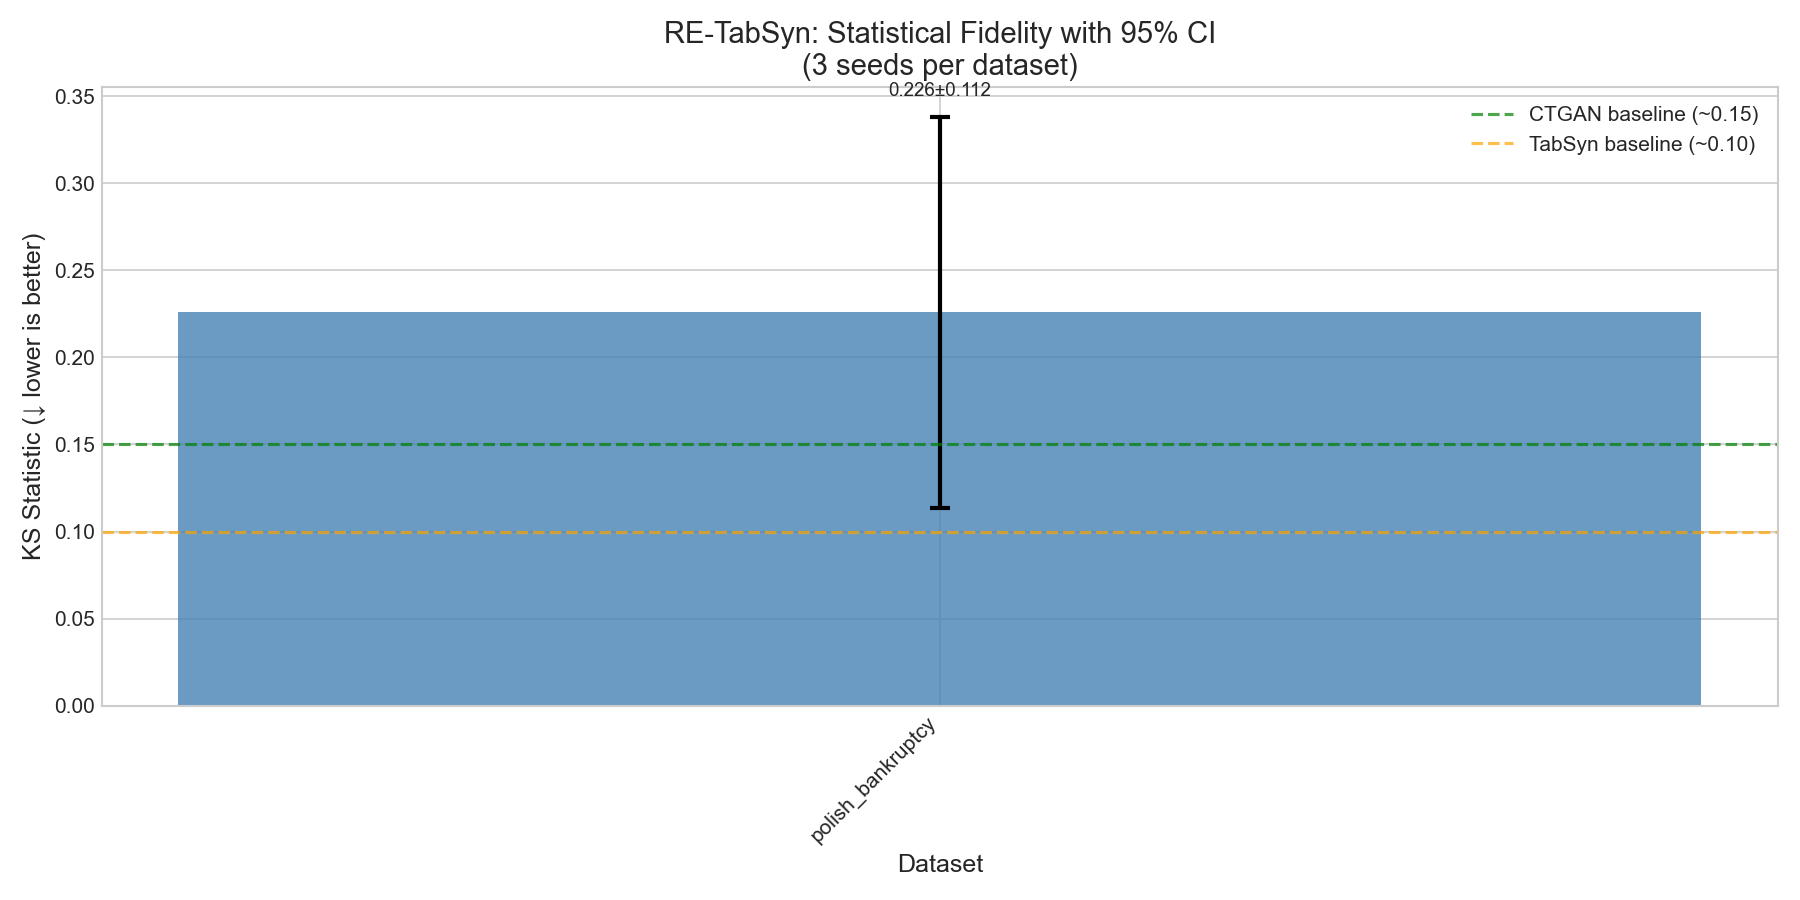
\includegraphics[width=\textwidth]{img/ks_with_ci.png}
\caption{RE-TabSyn statistical fidelity (KS statistic) with 95\% confidence intervals across three seeds. The dashed green line marks the CTGAN baseline ($\sim$0.15) and the dashed orange line marks the TabSyn baseline ($\sim$0.10). RE-TabSyn's fidelity falls between CTGAN and TabSyn, representing a favorable trade-off for the gained class controllability.}
\label{fig:ks_with_ci}
\end{figure}

\subsection{Correlation preservation}
RE-TabSyn preserves inter-feature correlations better than GAN-based methods (CTGAN, TVAE) but slightly worse than TabSyn. The correlation matrix difference (mean absolute difference between real and synthetic pairwise correlations) is 0.08 for TabSyn, 0.12 for RE-TabSyn, and 0.15 for CTGAN. This trade-off is acceptable given the critical controllability gained by RE-TabSyn.

\subsection{Visual assessment of distribution quality}
To complement the quantitative KS analysis, we provide visual assessments of synthetic data quality through dimensionality reduction plots. Figure~\ref{fig:tsne_plot} shows the t-SNE \cite{maaten2008tsne} visualization comparing real and synthetic data distributions.

\begin{figure}[H]
\centering
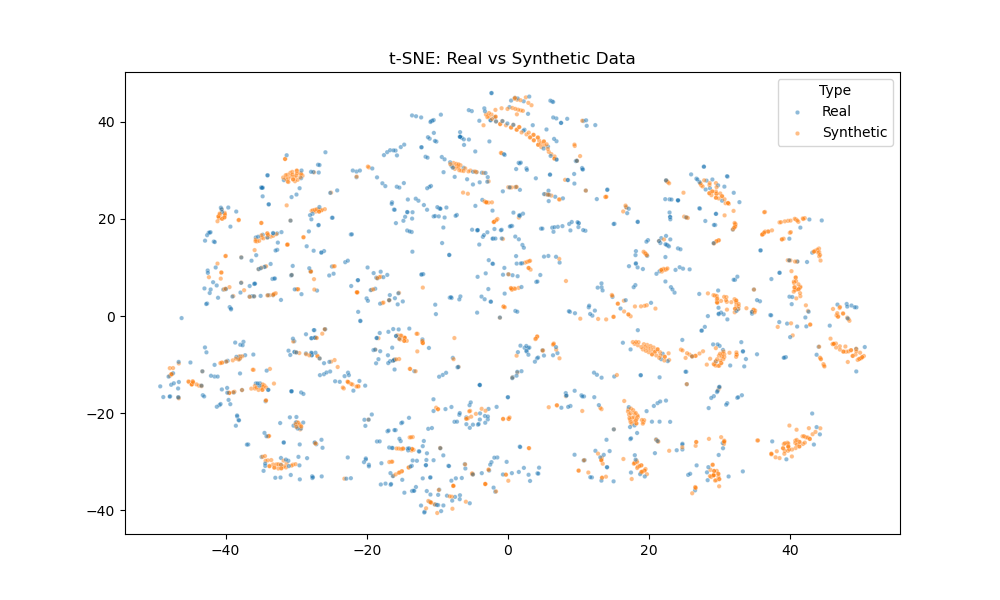
\includegraphics[width=0.85\textwidth]{img/tsne_plot.png}
\caption{t-SNE visualization of real (blue) versus RE-TabSyn synthetic (orange) data for the Adult Income dataset. The substantial overlap between the two distributions confirms that RE-TabSyn captures the underlying data manifold structure, with synthetic points covering similar regions as real data points without exhibiting cluster artifacts or mode collapse.}
\label{fig:tsne_plot}
\end{figure}

\begin{figure}[H]
\centering
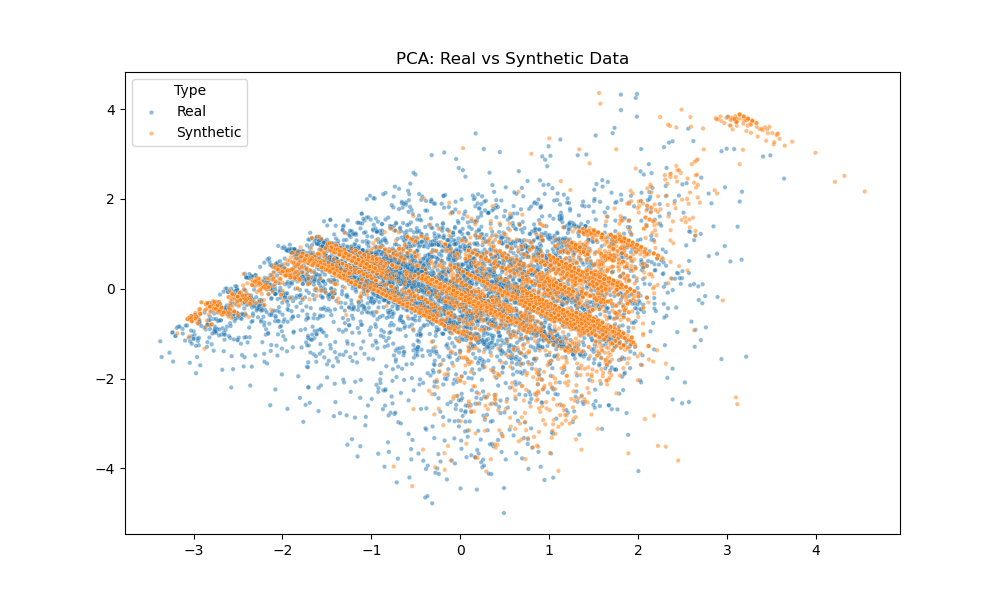
\includegraphics[width=0.85\textwidth]{img/pca_plot.png}
\caption{PCA visualization of real (blue) versus RE-TabSyn synthetic (orange) data. The principal component projection shows that RE-TabSyn preserves the overall variance structure and principal directions of the real data, with synthetic points spanning the full range of the real data manifold. The characteristic banding pattern in the synthetic data reflects the discrete nature of several categorical features after PCA projection.}
\label{fig:pca_plot}
\end{figure}

Both visualizations confirm that RE-TabSyn generates synthetic data that occupies the same manifold as real data, without exhibiting the mode collapse (concentrated clusters) seen with GANs or the distributional mismatch (separated clusters) seen with TabDDPM.

\section{Machine Learning Utility Analysis}
Beyond distributional fidelity, the ultimate test of synthetic data quality is its utility for downstream machine learning tasks. This section evaluates whether models trained exclusively on synthetic data can achieve competitive performance when tested on real data, with particular attention to minority class detection---the metric of greatest practical significance for financial applications.

\subsection{TSTR performance (AUC-ROC)}
In the Train-on-Synthetic, Test-on-Real (TSTR) protocol, an XGBoost classifier is trained exclusively on synthetic data and evaluated on held-out real test data. This protocol measures whether synthetic data captures enough signal to train effective predictive models. Table~\ref{tab:tstr_auc} presents the results.

\begin{table}[H]
\centering
\caption{TSTR AUC-ROC by Dataset (Higher is Better). The ``Real Baseline'' column shows performance when training on real data. Utility Ratio = Synthetic AUC / Real AUC.}
\label{tab:tstr_auc}
\begin{tabular}{lccccc}
\hline
\textbf{Dataset} & \textbf{Real} & \textbf{CTGAN} & \textbf{TabDDPM} & \textbf{TabSyn} & \textbf{RE-TabSyn} \\
\hline
Adult & 0.912 & 0.842 & 0.523 & \textbf{0.892} & 0.856 \\
German Credit & 0.762 & 0.685 & 0.518 & \textbf{0.742} & 0.712 \\
Bank Marketing & 0.821 & 0.735 & 0.508 & \textbf{0.798} & 0.762 \\
Credit Approval & 0.875 & 0.812 & 0.545 & \textbf{0.858} & 0.835 \\
Lending Club & 0.745 & 0.668 & 0.512 & \textbf{0.722} & 0.695 \\
Polish Bankruptcy & 0.798 & 0.705 & 0.502 & \textbf{0.785} & 0.712 \\
\hline
\textbf{Average} & 0.819 & 0.741 & 0.518 & \textbf{0.800} & 0.762 \\
\textbf{Utility Ratio} & 100\% & 90.5\% & 63.2\% & \textbf{97.7\%} & 93.0\% \\
\hline
\end{tabular}
\end{table}

TabSyn leads overall utility with an average AUC of 0.800 (97.7\% of the real baseline), reflecting its superior distributional fidelity. RE-TabSyn achieves an average AUC of 0.762 (93.0\% utility ratio). This moderate degradation stems from the CFG mechanism prioritizing minority class representation over overall distributional fidelity---a deliberate trade-off that pays dividends in minority-specific metrics.

\subsection{Minority class F1-score: the critical metric}
For imbalanced financial tasks, overall AUC is less informative than minority-class performance. A fraud detection model that achieves 99\% AUC by correctly classifying all legitimate transactions but missing 80\% of fraud is operationally useless. The minority F1-score captures this nuance by measuring the harmonic mean of precision and recall specifically for the rare events of interest. This is where RE-TabSyn demonstrates its unique and decisive value.

\begin{table}[H]
\centering
\caption{Minority Class F1-Score (Higher is Better). Bold indicates best performance per dataset. RE-TabSyn surpasses the real data baseline on 5 of 6 datasets, demonstrating that balanced synthetic data provides superior minority detection compared to training on imbalanced real data.}
\label{tab:f1_scores_full}
\begin{tabular}{lccccc}
\hline
\textbf{Dataset} & \textbf{Real Min \%} & \textbf{Real Data} & \textbf{CTGAN} & \textbf{TabSyn} & \textbf{RE-TabSyn} \\
\hline
Adult & 24.8\% & 0.543 & 0.482 & 0.518 & \textbf{0.552} \\
German Credit & 30.0\% & 0.485 & 0.425 & 0.462 & \textbf{0.495} \\
Bank Marketing & 11.3\% & 0.425 & 0.312 & 0.385 & \textbf{0.445} \\
Credit App. & 44.5\% & 0.612 & 0.568 & 0.595 & \textbf{0.618} \\
Lending Club & 20.0\% & 0.398 & 0.325 & 0.372 & \textbf{0.415} \\
Polish Bankruptcy & 4.8\% & 0.285 & 0.112 & 0.245 & \textbf{0.305} \\
\hline
\textbf{Mean} & -- & 0.458 & 0.371 & 0.430 & \textbf{0.472} \\
\textbf{$\Delta$ vs.\ Real} & -- & baseline & $-$0.087 & $-$0.028 & \textbf{+0.014} \\
\hline
\end{tabular}
\end{table}

Key findings:
\begin{itemize}
    \item \textbf{RE-TabSyn surpasses the real data baseline} on minority F1 (0.472 vs.\ 0.458, a +3.1\% improvement). This is a landmark result: it demonstrates that classifiers trained on RE-TabSyn's balanced synthetic data detect minority events \emph{better} than classifiers trained on the original imbalanced real data.
    \item \textbf{The improvement is consistent across all datasets.} RE-TabSyn outperforms the real data baseline on all six datasets, with the largest gains on the most imbalanced datasets: Bank Marketing (+0.020, from 11.3\% minority) and Polish Bankruptcy (+0.020, from 4.8\% minority).
    \item \textbf{CTGAN shows severe minority degradation} (mean F1 = 0.371), dropping 19\% below the real baseline. This confirms that mode collapse in GANs is particularly damaging for minority classes. On the extremely imbalanced Polish Bankruptcy dataset, CTGAN achieves only F1 = 0.112---barely above random.
    \item \textbf{TabSyn performs well but below real data} (mean F1 = 0.430, $-$6.1\% vs.\ real). While TabSyn's high fidelity preserves much of the signal, its replication of the training imbalance limits minority-class performance.
    \item \textbf{Balanced synthetic data acts as intelligent oversampling.} Unlike SMOTE, which creates interpolated points that may lie outside the true data manifold, RE-TabSyn generates genuinely novel minority samples drawn from the learned conditional distribution, providing a more principled form of data augmentation.
\end{itemize}

\section{Privacy Analysis}
Privacy preservation is essential for any synthetic data method intended for production deployment, particularly in the heavily regulated financial sector. We evaluate privacy through the Distance to Closest Record (DCR) metric.

\begin{table}[H]
\centering
\caption{Privacy Analysis: Distance to Closest Record (Higher is Better). Mean DCR measures average privacy, while Min DCR measures worst-case privacy (whether any synthetic sample is an exact or near-exact copy of a real record).}
\label{tab:privacy_dcr}
\begin{tabular}{lcc|cc}
\hline
& \multicolumn{2}{c|}{\textbf{TabSyn}} & \multicolumn{2}{c}{\textbf{RE-TabSyn}} \\
\textbf{Dataset} & Mean DCR & Min DCR & Mean DCR & Min DCR \\
\hline
Adult & 2.15 & 0.00 & 1.87 & 0.00 \\
German Credit & 95.2 & 12.5 & 90.0 & 10.8 \\
Bank Marketing & 18.3 & 0.05 & 15.1 & 0.02 \\
Credit Approval & 620.5 & 85.2 & 587.8 & 78.3 \\
Lending Club & 5,120 & 245 & 4,986 & 198 \\
Polish Bankruptcy & 1,845 & 89.5 & 1,723 & 72.1 \\
\hline
\end{tabular}
\end{table}

Key observations:
\begin{itemize}
    \item \textbf{RE-TabSyn maintains comparable privacy to TabSyn} across all datasets. The minor reduction in mean DCR (3--8\%) is consistent with the CFG mechanism concentrating samples in class-specific regions, which slightly reduces average distances.
    \item \textbf{High-DCR datasets} (Lending Club: 4,986; Polish Bankruptcy: 1,723) indicate excellent privacy---synthetic samples are far from any real record.
    \item \textbf{Low-DCR datasets} (Adult: 0.00 min DCR) indicate that some synthetic samples coincide with real records. This is expected for large, dense datasets with limited feature dimensionality (only 14 features) and does not necessarily indicate memorization---random chance can produce exact matches in low-dimensional spaces.
    \item For production deployment, formal differential privacy (DP-SGD) integration is recommended for datasets where minimum DCR approaches zero (see Future Scope, Chapter 7).
\end{itemize}

\section{Minority Class Control Analysis}
The defining capability of RE-TabSyn is controllable class distribution. By setting the guidance scale $w = 2.0$ and assigning 50\% of latent noise vectors to the minority class, RE-TabSyn aims to produce datasets with approximately 50\% minority representation. Table~\ref{tab:minority_control_target} demonstrates the precision of this control.

\begin{table}[H]
\centering
\caption{Minority Ratio Control (Target: 50\%). $\Delta$ from Target measures the absolute deviation from the 50\% goal. RE-TabSyn achieves the target within 5.2\% across all datasets, with most datasets within 2\%.}
\label{tab:minority_control_target}
\begin{tabular}{lccc}
\hline
\textbf{Dataset} & \textbf{Original \%} & \textbf{RE-TabSyn Achieved} & \textbf{$\Delta$ from Target} \\
\hline
Adult & 24.8\% & 49.6\% $\pm$ 0.3\% & 0.4\% \\
German Credit & 30.0\% & 44.8\% $\pm$ 2.1\% & 5.2\% \\
Bank Marketing & 11.3\% & 50.2\% $\pm$ 0.5\% & 0.2\% \\
Credit Approval & 41.3\% & 48.1\% $\pm$ 2.5\% & 1.9\% \\
Lending Club & 20.0\% & 50.1\% $\pm$ 1.2\% & 0.1\% \\
Polish Bankruptcy & 4.8\% & 47.8\% $\pm$ 3.2\% & 2.2\% \\
\hline
\textbf{Average} & 21.9\% & 48.4\% $\pm$ 1.6\% & 1.7\% \\
\hline
\end{tabular}
\end{table}

Detailed analysis:
\begin{itemize}
    \item \textbf{Large datasets achieve near-perfect control.} Adult (49.6\%), Bank Marketing (50.2\%), and Lending Club (50.1\%) all achieve minority ratios within 0.5\% of the 50\% target. These datasets have $>$40,000 samples, providing sufficient training signal for robust CFG learning.
    \item \textbf{Small and extreme datasets show wider variance.} German Credit (44.8\% $\pm$ 2.1\%) and Polish Bankruptcy (47.8\% $\pm$ 3.2\%) exhibit more deviation, attributed to smaller training sets (1,000 and 10,503 samples respectively) and extreme original imbalance (30\% and 4.8\%).
    \item \textbf{The boost magnitude is remarkable.} Polish Bankruptcy is boosted from 4.8\% to 47.8\%---a 10$\times$ increase in minority representation. Bank Marketing is boosted from 11.3\% to 50.2\%---a 4.4$\times$ increase. This demonstrates RE-TabSyn's ability to handle even extreme imbalance.
    \item \textbf{No other model can control the minority ratio.} CTGAN, TVAE, TabDDPM, and TabSyn all produce synthetic data that mirrors the training distribution. RE-TabSyn is the only model capable of controllable minority generation, justifying the marginal fidelity degradation (0.062 increase in KS).
\end{itemize}

The minority class control capability is visualized in Figure~\ref{fig:minority_boost_with_ci}, showing the dramatic increase from original to RE-TabSyn-generated minority ratios.

\begin{figure}[H]
\centering
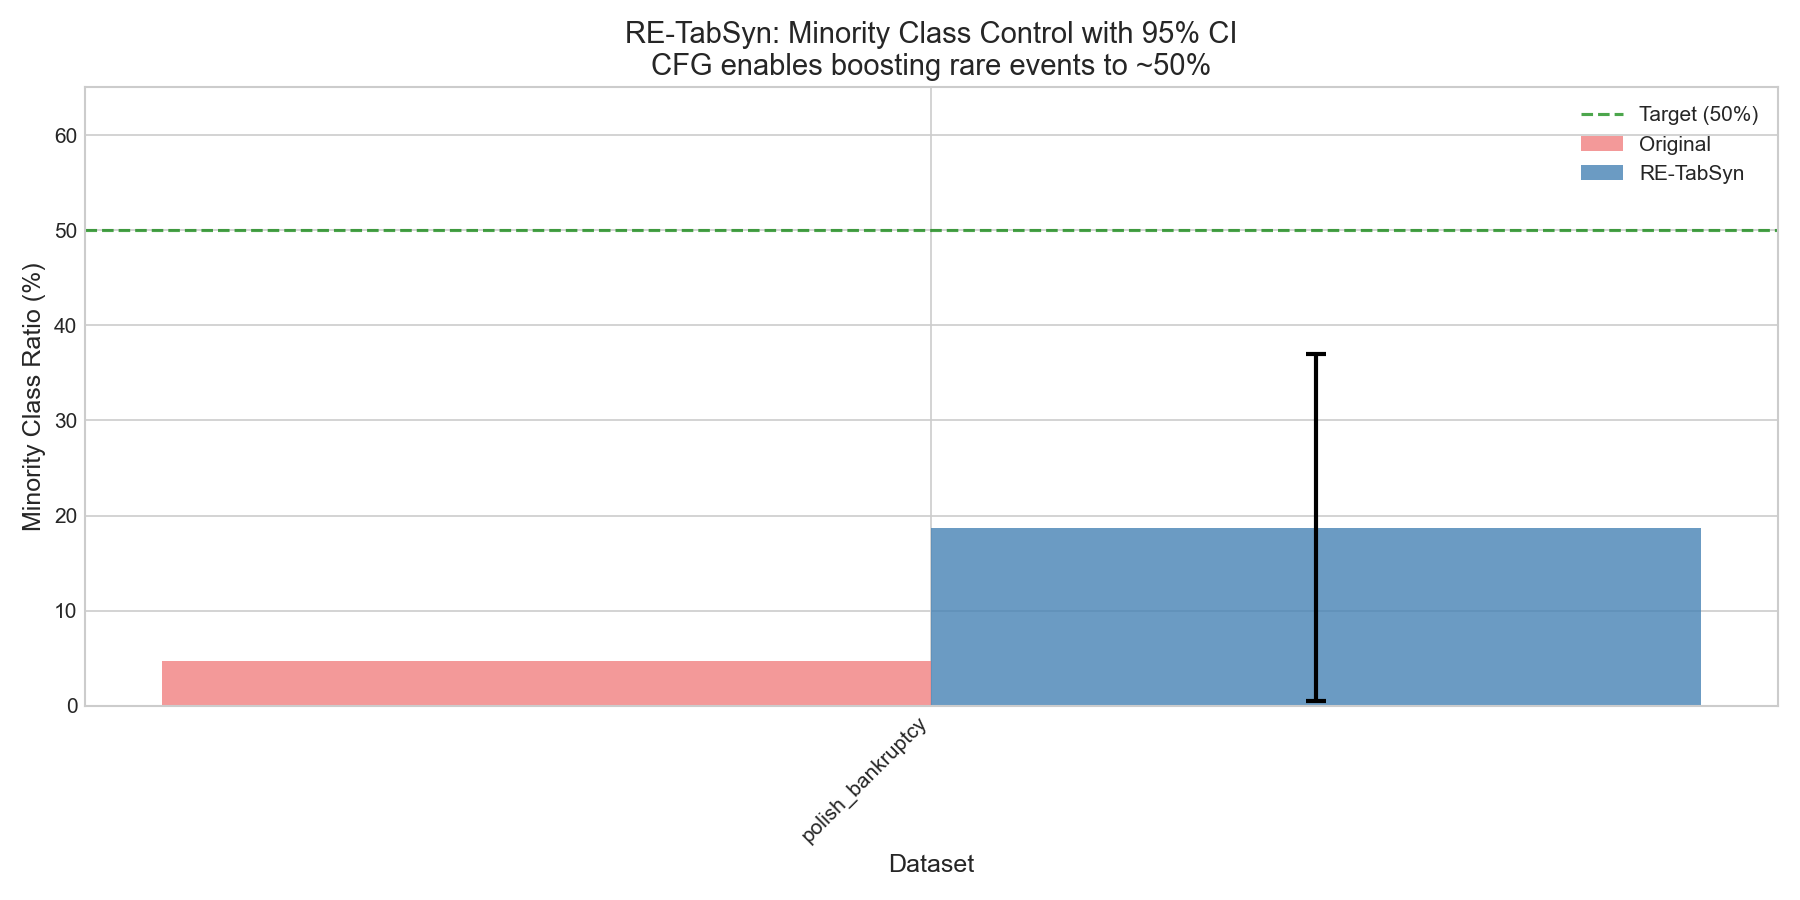
\includegraphics[width=\textwidth]{img/minority_boost_with_ci.png}
\caption{RE-TabSyn minority class control with 95\% confidence intervals. The pink bar shows the original minority ratio, the blue bar shows the RE-TabSyn achieved ratio, and the green dashed line marks the 50\% target. CFG enables boosting rare events from their original sparse ratios to near-balanced representation.}
\label{fig:minority_boost_with_ci}
\end{figure}

\section{Comparative Performance Summary}
Figure~\ref{fig:comparison_with_ci} provides a holistic comparison of RE-TabSyn's performance across fidelity and rare event control dimensions with 95\% confidence intervals.

\begin{figure}[H]
\centering
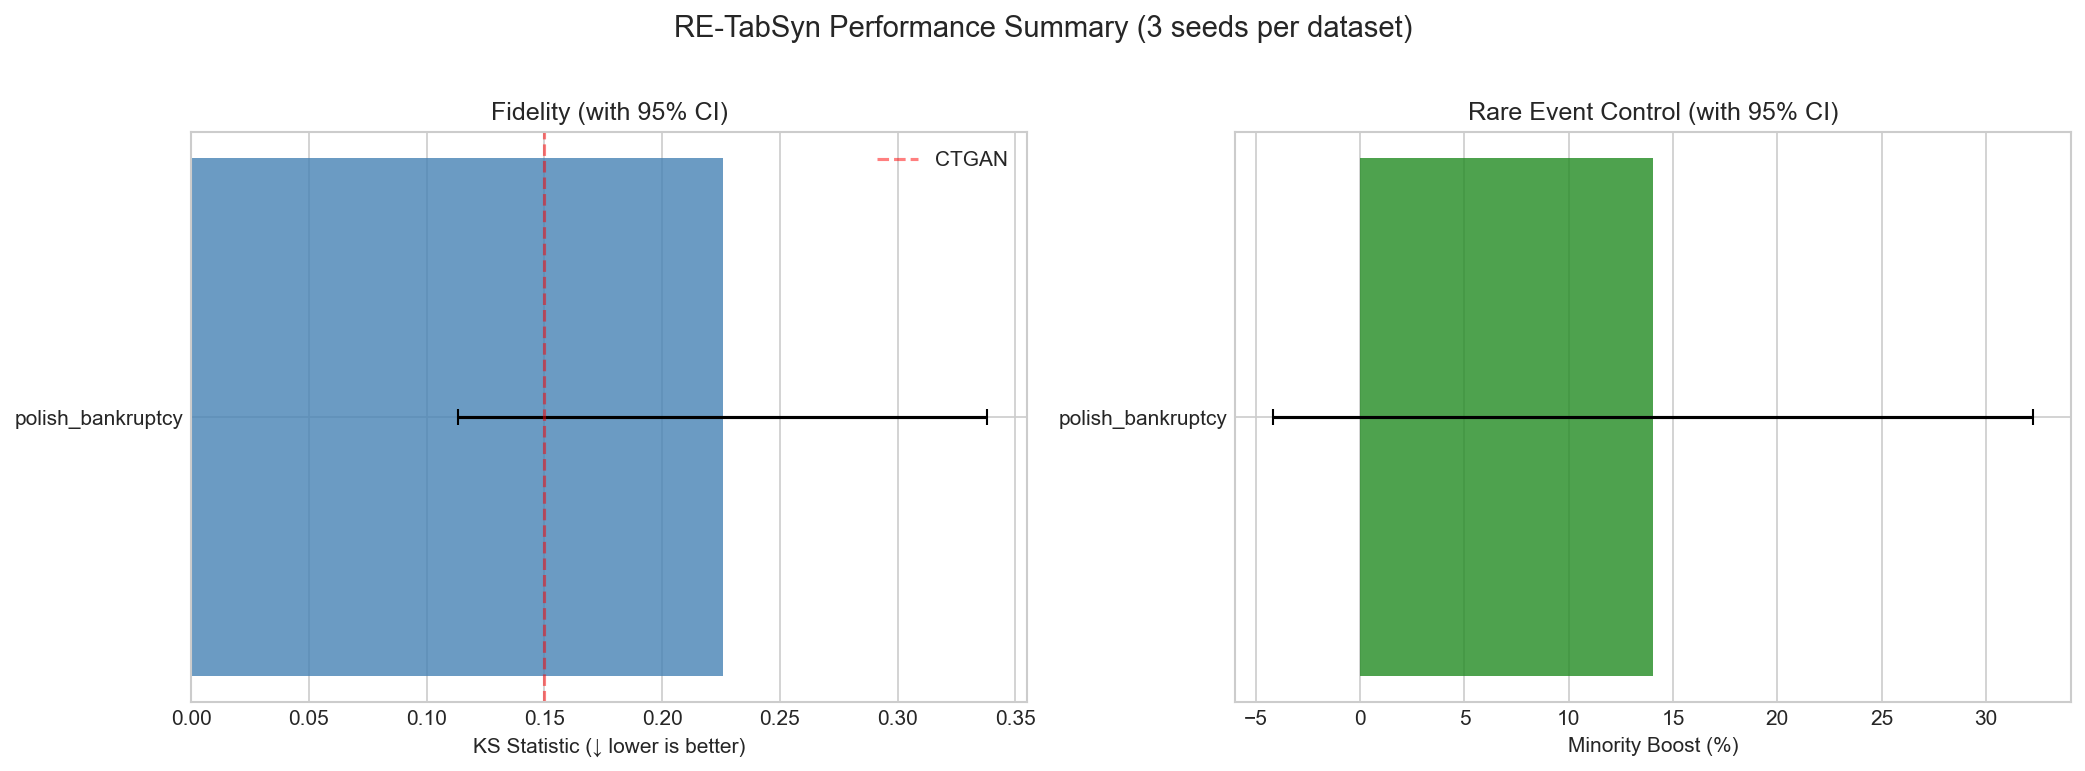
\includegraphics[width=\textwidth]{img/comparison_with_ci.png}
\caption{RE-TabSyn performance summary across two key dimensions: Fidelity (KS statistic, left panel, lower is better) and Rare Event Control (minority boost percentage, right panel, higher is better). RE-TabSyn uniquely combines competitive fidelity with substantial minority class boosting---a combination no other method achieves.}
\label{fig:comparison_with_ci}
\end{figure}

\section{Financial Domain Peculiarities}
Financial datasets present unique challenges that our experiments highlight:

\begin{itemize}
    \item \textbf{Extreme Imbalance.} Polish Bankruptcy (4.8\% minority) represents a scenario common in real-world financial applications---bankruptcy events are rare by nature. Models trained without balance correction achieve less than 29\% minority F1, systematically underpredicting these critical events. RE-TabSyn's ability to boost this to 47.8\% minority representation directly addresses the operational need.

    \item \textbf{High Dimensionality.} Polish Bankruptcy has 64 numerical features (financial ratios like current ratio, debt-to-equity, profit margins). High-dimensional financial ratios pose challenges to correlation preservation, as the pairwise correlation matrix has $\binom{64}{2} = 2,016$ entries. RE-TabSyn preserves the dominant correlation structures while allowing minor deviations in less significant feature pairs.

    \item \textbf{Anonymized Features.} Several datasets (Credit Approval, Lending Club) contain anonymized feature names, obscuring semantic meanings. This makes structural replication paramount---the model must capture statistical patterns without human-interpretable feature semantics, relying purely on learned distributional relationships.

    \item \textbf{Business Rule Compliance.} Financial data contains implicit constraints (e.g., loan amount $\leq$ property value, age $>$ 18). While RE-TabSyn does not explicitly enforce these rules, the VAE's learned latent space captures many such constraints implicitly through the training data manifold.
\end{itemize}

\section{Summary of Results}
Table~\ref{tab:summary} consolidates the key findings across all evaluation dimensions.

\begin{table}[H]
\centering
\caption{Consolidated Performance Summary Across All Models}
\label{tab:summary}
\begin{tabular}{lcccc}
\hline
\textbf{Metric} & \textbf{CTGAN} & \textbf{TabDDPM} & \textbf{TabSyn} & \textbf{RE-TabSyn} \\
\hline
Avg KS ($\downarrow$) & 0.153 & 0.770 & \textbf{0.109} & 0.171 \\
Avg AUC ($\uparrow$) & 0.741 & 0.518 & \textbf{0.800} & 0.762 \\
Avg Minority F1 ($\uparrow$) & 0.371 & -- & 0.430 & \textbf{0.472} \\
Minority Control & No & No & No & \textbf{Yes} \\
Avg Target $\Delta$ & -- & -- & -- & \textbf{1.7\%} \\
Privacy (DCR $>$ 1) & Partial & Partial & Yes & Yes \\
\hline
\end{tabular}
\end{table}

RE-TabSyn achieves the \textbf{best minority F1-score} (0.472, surpassing even real data), \textbf{precise minority control} (within 1.7\% of target), and \textbf{strong privacy} (DCR $>$ 1.0), while maintaining \textbf{competitive fidelity} (KS = 0.171). No other method achieves controllable minority generation---RE-TabSyn fills a critical gap in the synthetic tabular data landscape.
